\documentclass[twocolumn]{article}
\usepackage[utf8]{inputenc}
   \usepackage{fontspec}
   \setmainfont{Times New Roman}
%\usepackage[utopia]{mathdesign}
%\usepackage{mathptmx}
\usepackage[nottoc]{tocbibind}
\usepackage{amsmath}
\usepackage{amssymb}
\usepackage{amsfonts}
\usepackage{amsthm}
\usepackage{enumerate}
\usepackage{authblk}
\newcommand*{\everymodeprime}{\ensuremath{\prime}}
%\usepackage{algorithm}
%\usepackage{algorithmic}
%\renewcommand{\algorithmicrequire}{ \textbf{Input:}} %Use Input in the format of Algorithm
%\renewcommand{\algorithmicensure}{ \textbf{Output:}} %UseOutput in the format of Algorithm
\usepackage[linesnumbered,lined,ruled,vlined,commentsnumbered]{algorithm2e}

\newtheorem{theorem}{Theorem}[section]
\newtheorem{lemma}[theorem]{Lemma}
\newtheorem{proposition}[theorem]{Proposition}
\newtheorem{corollary}[theorem]{Corollary}
\newtheorem{definition}[theorem]{Definition}
\newtheorem{assertion}[theorem]{Assertion}

\usepackage[colorlinks,linkcolor=blue,anchorcolor=blue,citecolor=blue,bookmarks = True]{hyperref}
\usepackage{longtable}
\usepackage{multirow}
\usepackage{float}
%\usepackage{subfig}
\usepackage{subfigure}
\usepackage[titletoc]{appendix}
% \newcommand\appendix{\par
%   \setcounter{chapter}{0}%
%   \setcounter{section}{0}%
%   \gdef\@chapapp{\appendixname}%
%   \gdef\thechapter{\@Alph\c@chapter}}
\usepackage{booktabs}
\usepackage{graphics}
\usepackage{graphicx}
\usepackage[margin=25mm]{geometry}
\usepackage{color}
\usepackage{natbib}
\setcitestyle{authoryear,open={(},close={)}}
\usepackage{abstract}

\usepackage{graphicx}
\pagenumbering{gobble}
\usepackage{verbatim}

% Keywords command
\providecommand{\keywords}[1]
{
  \small    
  \textbf{\textit{Keywords:}} #1
}

\begin{document}
\title{Dynamic Model for Traffic Flow Prediction Using Updated Deep Residual Network}
\author[a]{Zeren Tan}
\author[b]{Ruimin Li}
\affil[a]{Department of Civil Engineering, Tsinghua University, Beijing 100084, China}
\affil[b]{Institute of Transportation Engineering, Tsinghua University, Beijing 100084, China\thanks{Email:lrmin@tsinghua.edu.cn}}


\date{May 2018}

\maketitle
\begin{abstract}
    Real-time traffic flow prediction can provide travelers with reliable traffic information to save people's time, and also assist traffic operation agencies in managing the traffic system effectively.  In this study, a dynamic prediction model was established by using an improved deep residual network(DRN). On the basis of the traditional DRN model, we  first integrated the input and output of the $i^{th}$ layer to the input of the $(i+1)^{th}$ layer and proved that each layer fit a simple function thereby reducing the error rate as the model was trained rapidly. Then, we used the concept of online learning on our model to update the pretrained model during the prediction process and rebuild our model with ongoing time series. The influence of the number of layers in our network was investigated by conducting experiments Results verified that performance was not necessorily improved when the network increased in depth. We also evaluated our network on both short and long time intervals. Result showed that our dynamic model demonstrated better accuracy than other state-of-the-art models when applied to traffic volume prediction in an expressway in Beijing. In addition, our dynamic model can perform better in practical applications. 
    
\end{abstract}
\keywords{Traffic flow prediction, Deep learning, Deep residual network, Dynamic model}
\section{Introduction}

Precise, rapid and timely traffic flow prediction is a major task of intelligent transportation systems (ITSs)\citep{deeptrend}. Making decisions based on real-time and predicted traffic flow is important to travelers, companies, and governments\citep{7244203}. Office workers need this type of information to schedule trips to their workplace. Traffic operation agencies can use the predicted traffic flow information to plan vehicle lanes\citep{yuan2011driving,wu2018hybrid}. However, despite the continuous research and development worldwide, accurate and short-term traffic flow prediction has remained a challenge to researchers for decades because of its stochastic and nonlinear characteristics. At the beginning of traffic flow prediction research,experts have mainly used linear methods, such as autoregressive integrated moving average (ARIMA) \citep{ARIMA}. These linear models, such as multivariable linear regression (MVLR)\citep{MVLR}, have been improved continuously and applied in traffic flow prediction, due to their simplicity and convenienc.  Despite the progress in linear models, prediction accuracy for nonlinear traffic flow still needs improvement. Therefore, finding powerful methods to predict accurate traffic flow is important for researchers.
\par
From approximately 40 years ago, machine learning algorithms have demonstrated good performance in many tasks such as prediction and classification. Thus, researchers have begun to use machine learning algorithms such as support vector regression (SVR) \citep{SVR} and k-nearest neighbor (k-NN) \citep{k-NN}, in traffic flow prediction. In spite of the increase in performance, these approaches fail to consider all characteristics of the traffic flow and obtain unsatisfactory performance due to the complexity of traffic flow. Thus, traffic flow prediction has attracted considerable attention from researchers from civil engineering, automation, industrial engineering, and computer science.
\par
In recent years, deep learning methods, which are a subset of machine learning methods, have shown remarkable performance in many computer science-related tasks, such as image classification, machine translation and speech recognition. An increasing number of researchers working in other fields, including civil engineering, have been inclined to use deep learning methods in structural damage detection\citep{lin2017structural,cha2017deep,cha2017autonomous,maedaroad,gaodeep}, concrete defect detection\citep{li2018unified}, pavement crack detection\citep{zhang2017automated}, transportation network reliability\citep{nabian2018deep}, traffic speed estimation\citep{liu2018short}, and real-time transportation management \citep{hashemiend}. 
  With the recent development in deep learning, traffic flow prediction has become an important research direction in the application of deep learning approaches, such as Recurrent Neural Network (RNN) \citep{RNN}, Long Short-Term Memory network (LSTM) \citep{LSTMtraffic}, Gated Recurrent Unit (GRU) \citep{gruTraffic}, Stacked Auto-Encoders (SAEs) \citep{SAE}, Deep Belief Network (DBN) \citep{huang2014deep}, and some other models \citep{vlahogianni2008temporal,stathopoulos2008fuzzy,ghosh2010random,tan2018dynamic,songmatch}. These models generally have complex network architectures that can capture the nonlinear nature of traffic flow. Hence, previous studies showed that these methods perform better in forecasting traffic flow than the traditional models in their experiments\citep{gruTraffic,LSTMtraffic,SAE,huang2014deep,RNN}. 
\par
RNN \citep{RNN}, LSTM \citep{LSTMtraffic} and GRU \citep{gruTraffic} are commonly used deep learning models. However, a considerable amount of time is required in training these models due to their complicated architectures. Experts are often required to stack less layers and set training epochs to a small number, there by reducing accuracy to a certain extent. Researchers can also use other techniques such as dropout to reduce the size of their training set, which will lead to a lower accuracy when the data set is not large enough. Therefore, using these models in practical applications is difficult. Previous studies have been based on static models, that is, models are not updated after training. However, realistic traffic flow condition is continuously updated and includes significant uncertainty. 
In addition, traffic flow data are periodic, with 1 day and 1 week as its periods\citep{tan2013tensor,tan2016comparison,wu2017robust}.
Furthermore, traffic flow is uncertain and changes all the time\citep{chen2018novel}. Therefore, we need to build a prediction mechanism for real-time updates and adapt to the continuously changing traffic flow status.
\par
In this study, we improved the traditional deep residual network (DRN)\citep{DRN} and proposed a Dynamic Improved Deep Residual Network (DIDRN) based prediction framework that will continuously update its training set when real data are available, and perform well in practical applications. The results showed that our model demonstrated robust performance in multistep prediction with a short amount of training time.
\par
The rest of this paper is organized as follows. Section  \ref{sec:LR} reviews the existing literature on short-term traffic flow prediction. Section \ref{sec:DRN} demonstrates the basic concepts of DRN. Section \ref{sec:improv} and Section \ref{sec:dyna} explain our process of further updating DRN and designing the dynamic model, respectively. Section \ref{sec:exre} presents experiments, compares our model's performance with commonly used models and analyzes the performance of our model in detail. Finally, section \ref{sec:confw} draw the conclusions and discusses future studies. Appendix lists all the algorithms used in this research.

\section{Literature Review}
\label{sec:LR}
Traffic flow prediction is a main task of ITSs. Research on traffic flow prediction has progressed considerably over the years. New models are constantly being proposed as the performance of these models also increases at the same time. 
\par
Traffic flow prediction has time-series\citep{cheng2012spatio}, regression\citep{dunne2011regime} or clustering problems\citep{xia2012clustering}. As methods improve, classical statistical inference methods have been replaced by alternative models such as Bayesian inference, multivariate time series models and neural networks\citep{vlahogianni2004short}.
\par 
The selection of traffic flow prediction model is a issue in traffic flow prediction\citep{abdulhai1999short}. 
Existing traffic flow prediction methods can be generally divided into the two main categories: of parametric methods non-parametric methods.
\par
Parametric methods such as ARIMA \citep{ARIMA}, Kalman-filtering\citep{chen2001use,chien2003dynamic,chien2003predicting,wang2006renaissance,van2008online,Jin2013,guo2014adaptive} and MVLR  \citep{MVLR} are often used by researchers. These approaches require predetermined model architecture and that the parameters of the model are calculated by using empirical data\citep{deeptrend}. Improved models based on ARIMA such as SARIMA were proposed in the 21st century\citep{williams2001multivariate,smith2002comparison,SARIMA,williams2003modeling,chandra2009predictions}. These models have simple and straightforward architectures but require a considerable amount of data and that the traffic condition is in a stationary process. Hence, these approaches are unsuitable when sufficient data are not available and their performance is unsatisfactory when the detected traffic flow of a certain location is not stable enough. In addition, parametric models require prior knowledge on finite sets of parameters. Thus, setting these parameters is a challenge.
Moreover, traffic flow data are random and uncertain. Therefore, those parametric approaches cannot perform well in the majority of these cases.  They are also limited both theoretically and practically.
\par
The structure and parameters of nonparametric models need not to be fixed in advance\citep{ma2015long}.
At the beginning of the 21st century, researchers have focused on non-parametric approaches such as k-NN \citep{k-NN},Bayesian Network approach \citep{1603558,castillo2008predicting,sun2006bayesian}, SVR \citep{SVR,wu2004travel,asif2014spatiotemporal}, random forests regression (RF) \citep{RF}, gradient boosting regression \citep{GB}.
These machine learning approaches also require a large amount of data and may not be the optimal choice when sufficient data are not available \citep{k-NN,sun2006bayesian}. As \citet{sun2006bayesian} mentioned in their paper, their Bayesian network model can work well when data are incomplete but it is not the best choice to use their model when some abnormal scenarios occur. \citet{zheng2006short} introduced a Bayesian combination method (BCM) \citep{petridis2001bayesian} for traffic flow prediction. However, as \citet{wang2014new} pointed out, BCM does not consider the relevance between historic traffic flows and current traffic flows. Therefore, this model is not recommended for traffic flow prediction because traffic flow is a type of sequential data thereby indicating that current data are related to historical data. However, researchers from many fields, including transportation, have used Artificial Neural Networks due to their excellent performance in capturing nonlinearities and its more flexible structure, generalization ability, learning ability and adaptability \citep{DBLP:conf/isnn/LiL09b,li2011incorporating,karlaftis2011statistical,ma2015long}.
\par
Applications of neural networks in traffic flow prediction have been extended largely from simple multilayer perceptrons \citep{clark1993use}, to advanced structures, such as time-delayed recurrent neural networks\citep{abdulhai1999short}.
\par
With the rapid development of deep learning, many deep learning models have been proposed by computer scientists. Thess type of model can represent the complex features of traffic flow without prior hypothesis \citep{lv2015traffic,chen2018novel}. Developing a neural network model by adding layers and feeding your data into the network are required. Prior knowledge is unnecessary in depth when training and predicting are conducted. However, theoretical evidence shows that a single-layer neural network can represent any Borel measurable function\citet{hornik1989multilayer}. Many powerful deep learning models, such as SAE \citep{SAE}, DBN \citep{huang2014deep}, RNN \citep{RNN}, LSTM \citep{LSTMtraffic,ma2015long}, GRU \citep{gruTraffic,zhang2018combining} and Fuzzy Deep Convolution Neural Network(FDCN) \citep{chen2018novel}, were introduced in traffic flow prediction and showed superior performance compared with traditional models. 
\citet{SAE} proposed a greedy layer-wise unsupervised learning algorithm to train the model thereby reducing the training time significantly without accuracy loss.
 \citet{LSTMtraffic} proposed a model called LSTM RNN for short-term traffic flow prediction and their results achieved higher accuracy than classic models such as SVM. \citet{gruTraffic} proposed GRU NN for traffic flow prediction and their results showed that GRU and LSTM outperformed ARIMA. \citet{chen2018novel} developed a fuzzy deep learning model called FDCN. Apart from demonstrating powerful representing capability, their results also showed stability in terms of root mean sqaure error(RMSE) in performing mmultistep forecasting. 
\par
Sequential data are correlated with data in the context. However, common neural networks cannot capture this correlation among data. In the 1990s, RNN \citep{RNNraw} was developed to solve this problem. Although RNN can capture correlation among data, this correlation is soon forgotten, that is, this neural network does not have long-term memory \citep{zhao2017lstm,ma2015long}. Hence, if data are strongly correlated and historical data have a remarkable influence on consequent data even after a long time, choosing RNN as the training model is not recommended.
In 1997, long short-term memory (LSTM) networks \citep{LSTM} were proposed and set accuracy records in various application domains. LSTM can remember correlation for a long time and thus demonstrates outstanding performance in sequential modeling.
However, both RNN and LSTM are difficult to train because the architecture of these models is too complex \citep{lei2017training}. Researchers often take hours or even days to train these models so training model is time-consuming especially when the the dataset is very large.  Despite their good performance, using them in practical scenarios is sometimes impossible. 
To reduce mathematical operations and total running time, gated recurrent unit (GRU) was developed by \citet{gruTraffic}. Unfortunately, in practice, although GRU can reduce training time, the cost is still high. In addition, \citet{lstmcomparison} successfully compared variants of LSTM by conducting a large-scale study on many different datasets and found that these LSTM based methods are all the same and none of its modifications improved performance significantly.
\par
Apart from RNN and LSTM, researchers have also used some other deep learning models. \citet{ELM} proposed a novel double deep ELMs(Extreme Learning Machines) ensemble system (DD-ELMs-ES)  which used three deep ELM models as basic models and their model demonstrated better generalization performance than some state-of-the-art algorithms. However, their model only focused on one-step forecasting. \citet{deeptrend} implemented DeepTrend which decomposed original traffic flow data into trend and residual components. They demonstrated that DeepTrend could noticeably improve prediction performance and outperform many traditional models as well as LSTM. \citet{DBEN} proposed a deep belief echo-state network (DBEN) to address the problem of slow convergence and local optimum in time series prediction. Their experimental results demonstrated that DBEN has good performance in learning speed and short-term memory capacity. However, a large number of parameters exist in their model, thereby indicating difficulty in parameter tuning.
\par
\citet{DRN} proposed deep residual network (DRN) in ImageNet Large Scale Visual Recognition Challenge (ILSVRC). Their model substantially outperformed other models and won the first prize in this competition. Typically, training difficulty increases as the number of layers also increases in network, and the problem of gradient vanishing will arise in the mean time.  Their model performed training easily and solved this problem effectively even when the deep neural network is several times deeper than other networks.  For a normal deep neural network, the maximum depth that people has been less than 100. However, for DRN, a network with several hundred layers can be easily created and training can be conducted in a short time. Thus, we were motivated to apply DRN concepts to traffic flow prediction. Accordingly, we improved the architecture of DRN and its effectiveness. Section~\ref{sec:exre} illustrates our results.

\par
The main contributions of this study are as follows:
\begin{itemize}
    \item We apply and improve deep residual network in traffic flow prediction.
    \item We consider practical applications and propose a dynamic model called DIDRN.
    \item Results show that our model is more powerful than other commonly used models.
\end{itemize}

\section{Model Development} \label{sec:method}
In this section, we first introduced the concept of a normal neural network works. We then explained the structure of DRN and quoted a hypothesis proposed in \citep{DRN}. In the final subsection, the structure of DIDRN was proposed.

\subsection{Original DRN}\label{sec:DRN}

When the popularity of deep learning began to increase, experts simply stacked layers and assumed that deeper is better. The network was given an input $x$ and the intermediate layers fit a map $H$ to obtain the final output $H(x)$. As they believe deeper networks could have better performances, they stack more layers to fit the desired map $H$ and expect to obtain a higher accuracy. However, when the depth of the network increased, both training and test accuracy get saturated, that is, degradation occurred\citep{DRN}. Figure \ref{fig:com_nn} shows the architecture of a simple stacked neural network.
\begin{figure}[H]
\centering
    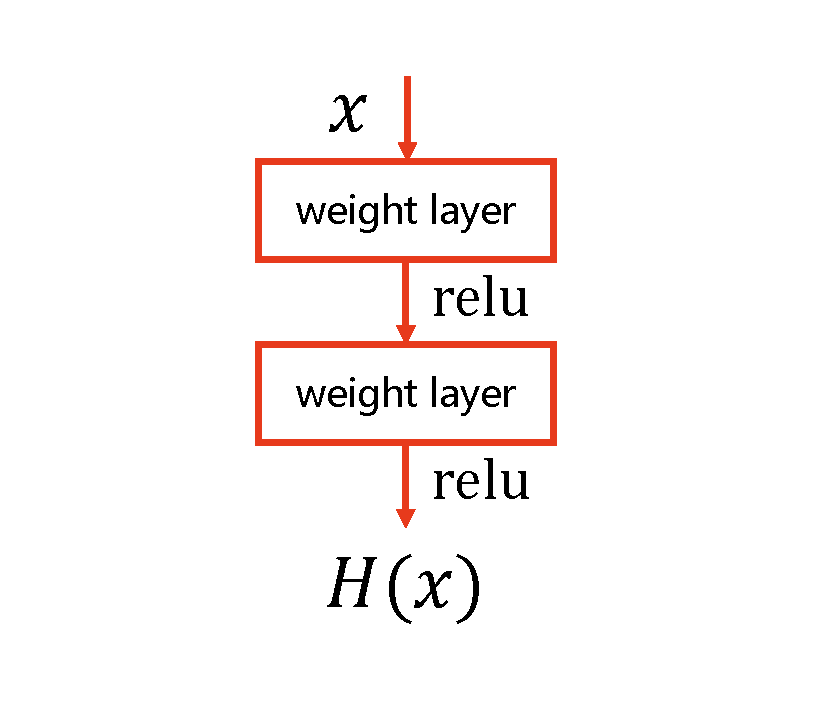
\includegraphics[width = 6cm]{fig/common_NN}
    \caption{Architecture of common neural network}
    \label{fig:com_nn}
\end{figure}
\par
DRN was proposed to solve degradation problem. Instead of expecting that each stacked layer will fit into a desired mapping directly. These layers fit the function via residual mapping.
\par
Hence, assuming that the network is expected to fit $H(x)$, \citet{DRN} let the sacked layer fit another mapping $F(x) = H(x) - x$ . Then the desired mapping $H(x)$ could be replaced by $F(x)+x$.
\par
They hypothesized that fitting the residual mapping $F(x)$ was easier than the original mapping $H(x)$. If the optimal mapping is identity, then it would be easy to make the residual be zero. Figure \ref{fig:res_nn} shows the idea stated above.
\begin{figure}[H]
    \centering
    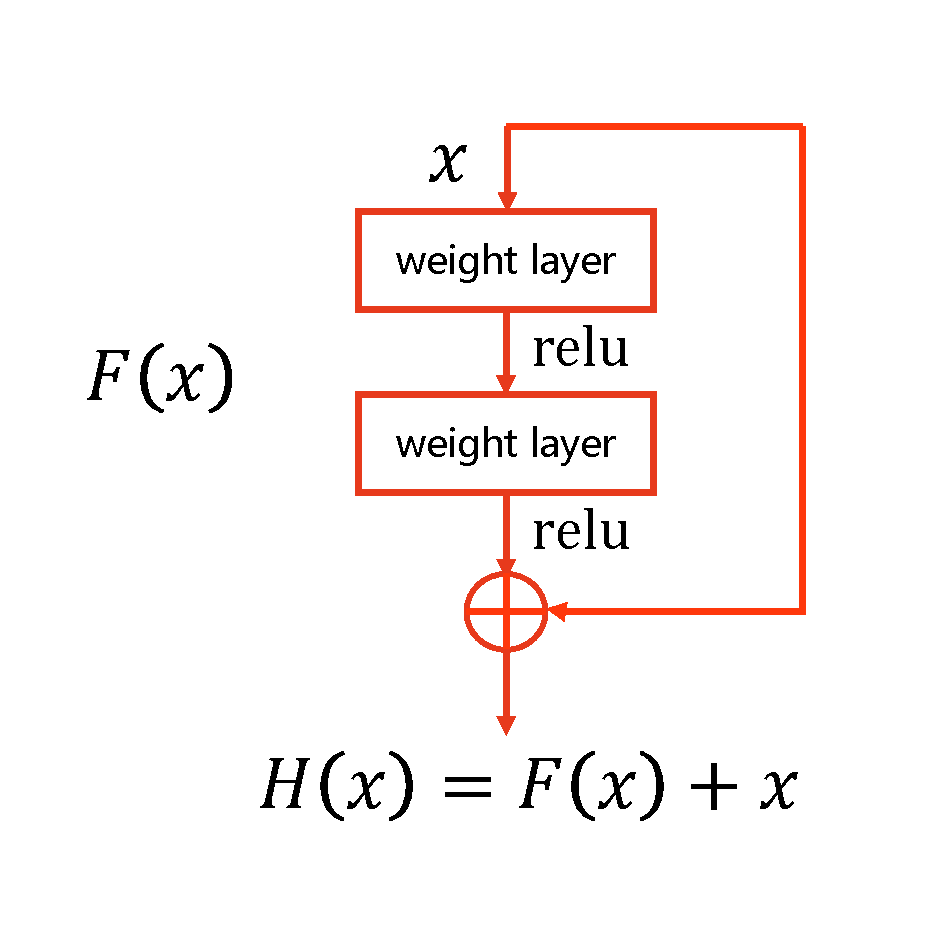
\includegraphics[width = 6cm]{fig/residual_NN.pdf}
    \caption{Architecture of residual neural network}
    \label{fig:res_nn}
\end{figure}

\par
This simple change made a remarkable difference as traning the network becomes easy. Deep residual network has helped Kaiming et.al. win first prize in the ILSVRC classification competition and many other competitions. Prior to DRN, the award-winning network of ILSVRC had a maximum number of 32 layers. However, when DRN participated in this competition, it had 152 layers with a significant increase in accuracy.

\subsection{Updated DRN} \label{sec:improv}
In the training process of neural networks, the estimated function is derived from the objective function to achieve computation accuracy. Therefore, the accuracy will decrease due to information loss.
To preserve more information when information is transferred among layers and thus obtain high accuracy, we further improved the architecture of DRN and used it in traffic flow prediction. Figure \ref{fig:imp_nn} shows the architecture of our improved network.
\begin{figure}[H]
    \centering
    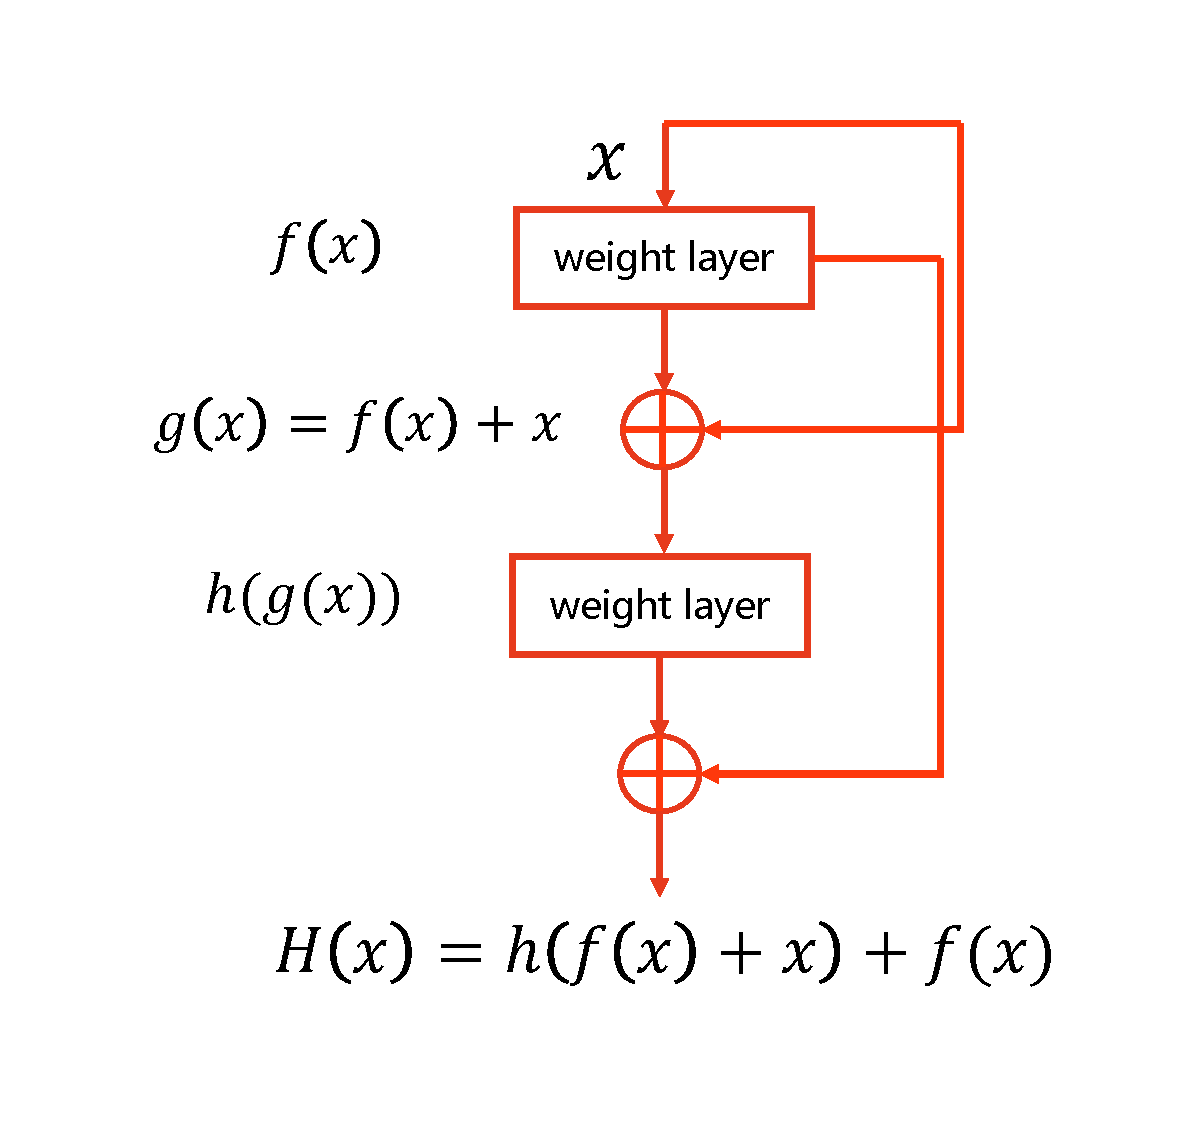
\includegraphics[width = 6cm]{fig/improved_NN.pdf}
    \caption{Our improved residual network}
    \label{fig:imp_nn}
\end{figure}

\par
The training process of our improved network is as follows: 
\begin{itemize}
    \item Denote the input as $x$, and the first layer fits the function $f(x)$. 
    \item Add these two outputs together to obtain $g(x) = f(x) +x $. 
    \item The second layer considers $g(x)$ as the input and maps it into $h(g(x))$. 
    \item Similarly, add the output of the first layer $f(x)$ and the output of the second   layer $h(g(x))$ to obtain $H(x) = h(f(x)+x) + f(x)$. 
\end{itemize}
\par 
From these steps, the task of fitting a complex function $H(x)$ was divided into fitting two simpler mappings $f$ and $h$, respectively. According to the hypothesis of \citet{DRN}, the layers will work more efficiently because fitting these two simple mappings is easy, thereby reducing the error rate in fitting these two mappings and subsequently reducing the overall error rate.

\subsection{Dynamic Model} \label{sec:dyna}
In practice, a traffic operation center would not use this model in the exact place where our training data come from, that is, our model needs to be transferred easily among different places. In addition, traffic flow on a specific road could change over time. Hence, the traffic flow after 1 month or 1 year may have significant difference with the existing situation, especially in rapidly developing cities.  In the DRN model, weights and parameters were obtained by using the previous training data. These weights and parameters could fit the previous data well but it may not fit the new data well, that is the previous model may not perform well by using the new data. Therefore, simply using the existing model with only one training process to predict traffic flow without any improvement was unreasonable. The old model could not be expected to perform well when the traffic flow changed significantly. Hence, traffic flow prediction models should be updated constantly. On the basis of these ideas, we designed a dynamic model based on the improved DRN.
\par
We used the basic idea of incremental learning to update the pretrained model and implement the dynamic model. 
\par
The complete process is as follows:
\begin{enumerate}[Step 1]
    \item\label{step:1} We use the collected data to pretrain the basic mode    l.
    \item\label{step:2} We use our model to predict traffic flow.
    \item\label{step:3} After some time,the basic model complete the predict    ion steps, and we obtain some new real data.
    \item\label{step:4} We combine these new data with the existing training     set into a new training set and use this new training set to retrain ou    r model.
    \item\label{step:5} Repeat Step \ref{step:2}-Step \ref{step:4}.
\end{enumerate}
\par
Figure \ref{fig:steps} shows this process.

\begin{figure}
    \centering
    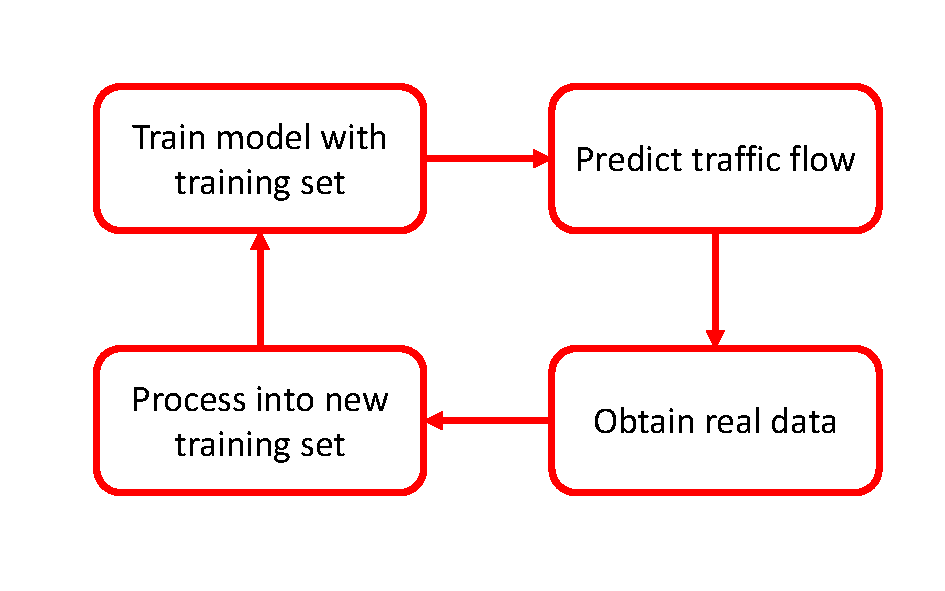
\includegraphics[width=8cm]{fig/Steps.pdf}
    \caption{Dynamic Model}
    \label{fig:steps}
\end{figure}

\par
With these steps, the model will be continuously updated by absorbing new data. Therefore, the proposed dynamic model satisfied the practical conditions better and obtained more accurate predictions than the existing model.
\subsection{Model Implementation}
In this section, we will present the entire process of implementing the model in detail.
\par
The process is divided into the following steps:
\begin{enumerate}[Step 1]
\item\label{step:11} Denote the raw data as $R$, which is a column vector of $R^n$. 
\[
R=\begin{bmatrix}
R_1\\
R_2\\
\vdots\\
R_n
\end{bmatrix}
\]
\par
Assume that trend characteristics exist in traffic flow data. Thus, we subtract the adjacent data to obtain the difference vector $D=[D_1, D_2, \cdots, D_{n-1}]$, where
\[
D_i = R_{i+1}-R_i \quad i = 1,2,\cdots,n-1
\]
\item\label{step:22} However, we cannot directly apply supervised learning to $D$. Hence, we further process our data into supervised data. 
\par
First, select the time-step, which represents the number of previous data points that were used to predict the next data point. After parameter tuning, we choose 1 as our time-step, that is, time-step = 1. 
\par
Then we denote $X$ as the feature and $Y$ as the data to be predicted. $X$ and $Y$ are defined as follows.
\[
X = \begin{bmatrix}
X_1\\
X_2\\
\vdots\\
X_n
\end{bmatrix}
\quad
Y = \begin{bmatrix}
Y_1\\
Y_2\\
\vdots\\
Y_n
\end{bmatrix}
\]
where
\[
X_1 = 0\quad X_i = D_{i-1},i= 2,3,\cdots,n-1
\]
\[
Y_i = D_{i}, i = 1,2,\cdots,n-1
\]
\par
Then we obtain the entire data set as follows:
\[
\begin{bmatrix}
X_1&Y_1\\
X_2&Y_2\\
\vdots & \vdots\\
X_{n-1} &Y_{n-1}
\end{bmatrix}
\]

\item\label{step:33} Normalization, which is a simple approach often used in developing deep learning models and performing experiments, is conducted to accelerate training and prediction. Elements in $D$ can be positive or negative. Thus, $X$ and $Y$ are scaled into $(-1,1)$. We define the following obtained vectors as $scaled\_X$ and $scaled\_Y$. 
\[
scaled\_X = \begin{bmatrix}
scaled\_X_1\\
scaled\_X_2\\
\vdots\\
scaled\_X_{n-1}
\end{bmatrix}
scaled\_Y = \begin{bmatrix}
scaled\_Y_1\\
scaled\_Y_2\\
\vdots\\
scaled\_Y_{n-1}
\end{bmatrix}
\]
\par
where
\[
scaled\_X_i = 2\frac{X_i - X_{min}}{X_{max}-X_{min}}-1
\]
\[
scaled\_Y_i = 2\frac{Y_i - Y_{min}}{Y_{max}-Y_{min}}-1
\]
\par
and
\[ 
scaled\_X_i \in (-1,1), i = 1,2,\cdots,n-1
\]
\[
scaled\_Y_i \in (-1,1), i = 1,2,\cdots,n-1
\]
\par
Then the data set is transformed as:
\[
\begin{bmatrix}
scaled\_X_1 & scaled\_Y_1\\
scaled\_X_2 & scaled\_Y_2\\
\vdots&\vdots\\
scaled\_X_{n-1} & scaled\_Y_{n-1}
\end{bmatrix}
\]
\item\label{step:44} During prediction, we invert Step \ref{step:11} and Step \ref{step:33} to obtain the final prediction data.
\end{enumerate}
All algorithms (Algorithm~\ref{alg:a1} $\sim$ Algorithm~\ref{alg:a5}) used to implement the entire process are presented in Appendix~\ref{algorithms}


\section{Experiments and Results} \label{sec:exre}
\subsection{Data Source}
Our data were obtained from the traffic detectors located in the ring roads of Beijing, China. Basic traffic flow data are collected via 14 microwave detectors, which were numbered as 2010, 2011, 2013, 2023, 2030, 2033, 2052, 3034, 3035, 4004, 4005, 4050, 4051, and 5062. The time interval in these traffic flow data was 10 minutes. 
 The time span is 61 days from June $1^{st}$, 2013 to July $31^{st}$,2013. Therefore, there are 8784 data points for each detector. For data from each detector, we use the first 7200 pieces of the entire data set as training data and the rest as test data. The detected traffic flow is loaded as input and finally we get the predicted traffic flow at specified time points as output. The results verify the feasibility and effectiveness of our proposed model.

\subsection{Performance Indexes}

\par 
Rooted Mean Square Error (RMSE), Mean Absolute Percentage Error (MAPE) and Mean Absolute Error (MAE) are chosen as performance indexes to evaluate the performance of these four models.
\par 
RMSE, MAPE and MAE were defined as follows:
\[
RMSE = \sqrt{\frac{1}{n}\sum_{i=1}^{n}(\hat{y}-y)^2}
\]
\[
MAPE = \frac{1}{n}\sum_{i = 1}^{n}\frac{|\hat{y_i} - y_i|}{y_i} \times 100\%
\]
\[
MAE = \frac{1}{n}\sum_{i=1}^n|\hat{y}-y|
\]
where $y_i$  and $\hat{y_i}$ refer to the real and forecasted values.
\par
We use these three performance indexes to evaluate the following aspects of the selected models: 1) absolute error and 2) relative error. RMSE and MAE represented the deviation from the predicted values and the detected values. They also increase with the increase in the range of data. MAPE measured the deviation from the predicted values and the ground truth values. This index determined percentage error, which was not related to the range of our data. 


\subsection{Performance Analysis}
\par
To analyze the efficiency of our model, the following experiments have been carried out.
\begin{enumerate}[(a)]
    \item The performance of DIDRN in terms of the different number of layers was inspected to determine the changes in prediction accuracy when the number of layers changed as shown in Section~\ref{subsubsec:layers}.
    \item The performance of different models in short-term traffic flow prediction was explored as shown in Section~\ref{subsubsec:short}.
    \item The performance of DIDRN under different prediction time intervals was investigated, as shown in Section~\ref{subsubsec:further}. Concretely, we increase the time interval gradually from 10 minutes to 7 days to evaluate the stability of our model, analyze its performance and determine the optimal model in predicting traffic flow.
\end{enumerate}
\par
The experiments were performed on a laptop with @2.60 GHz processor, 8.0 GB RAM and NVIDIA GeForce GTX 960M. The models were coded via Python 3.6 with Keras and TensorFlow frameworks and compiled by using the Anaconda Jupyter Notebook.

\subsubsection{Impact of the Number of Layers}\label{subsubsec:layers}
\par
First, the input dimension should be determined, that is the number of data points we input to the models is considered one input point. For example, if the input dimension was chosen as 5, then the models used 5 data points to predict the traffic flow of next time point. After parameter tuning, the input dimension was chosen as 1. 
\par
As previously mentioned, when the depth of the network increases, the accuracy rate will first increase and then decrease. To verify this, experiments were performed on DIDRN with different numbers of layers. In these experiments, the chosen time interval was 10 minutes.
Figure~\ref{fig:layer} shows that a shallow network obtained relatively good performance, but a deep network increases the error rate.  When the network had over 40 layers, the error rate increased significantly. We selected small numbers and found that the error rate was the lowest among all experimented numbers when the number was equal to 16. Although a similar error rate was still obtained when the number was 36, the training time became longer as the network became deeper. When the number of layer exceeded 40, the error rate exhibited a clear trend of increasing and that was significantly higher than that when the network was shallow. Hence, we choose less points in our experiments and the result thoroughly verify the reported problem in \citep{srivastava2015highway,he2015convolutional,DRN}.

\begin{figure*}[h]
    \centering
    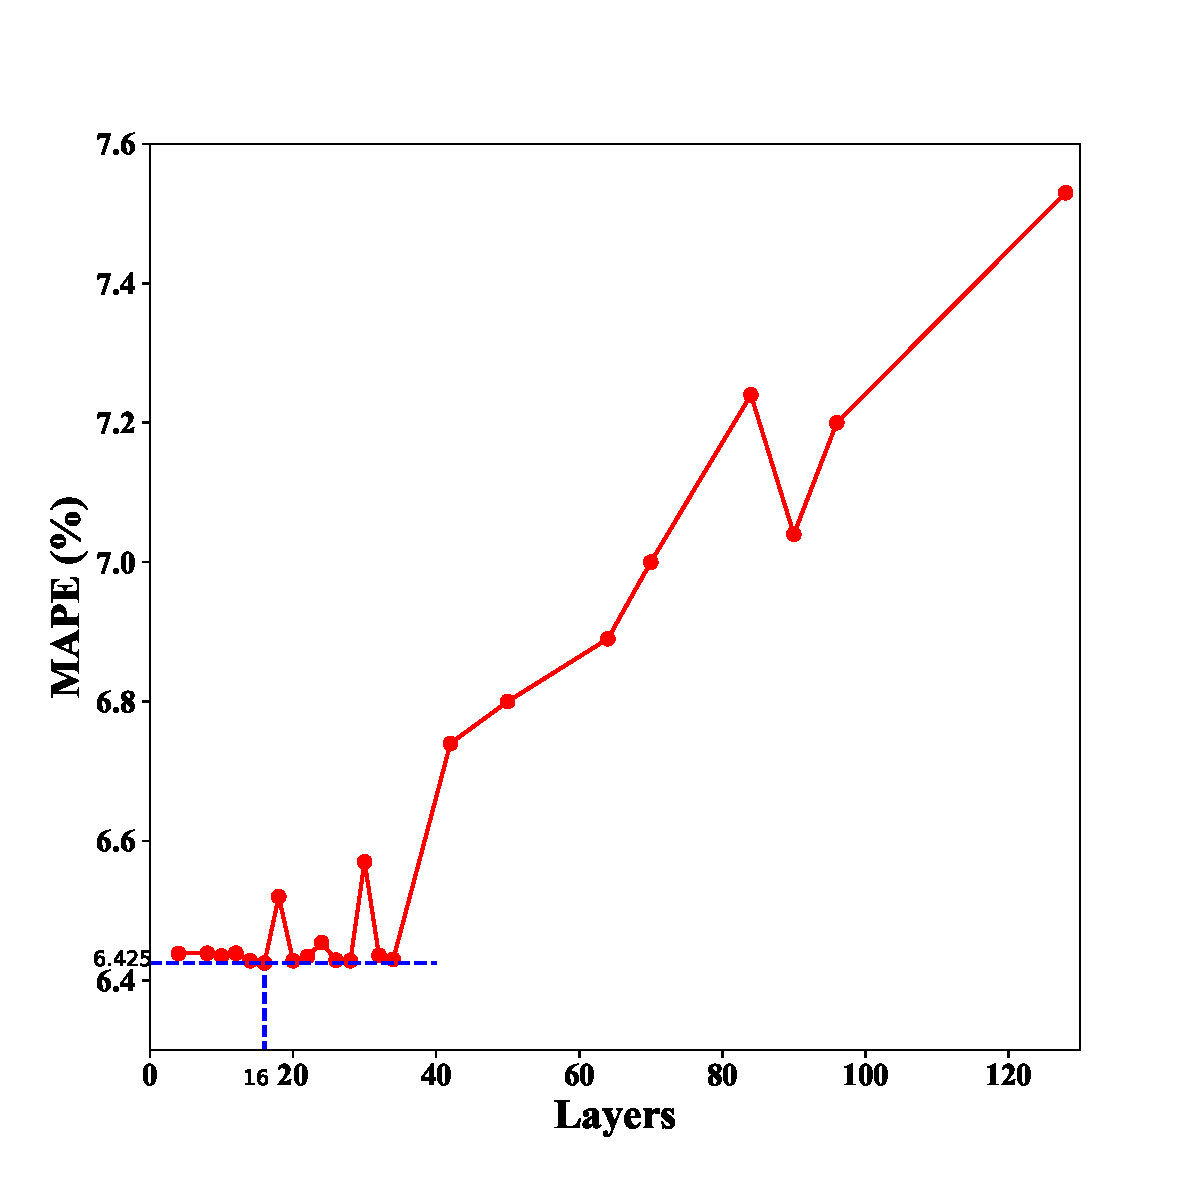
\includegraphics[height = 6.5cm]{Figure/layers.pdf}
    \caption{Impact of number of layers}
    \label{fig:layer}
\end{figure*}


\subsubsection{Short-term prediction}\label{subsubsec:short}
\par
To evaluate the efficiency of our proposed model, we performed several experiments on our proposed model and other similar models, including the one layer LSTM, deep LSTM, and DRN. From the result in Section~\ref{subsubsec:layers}, except for those of the one layer LSTM, the three other models have 16 layers. To change the input dimension into the output dimension, we added some layers to both DRN and DIDRN but maintained both should still have 16 layers in total.

\par 
We first used these models to predict the short-term traffic flow. Concretely, the interval of time points was 10 minutes. That is, we used the previous traffic flow to predict the traffic flow 10 minutes later. 
\par
Table \ref{tab:1} and Figure \ref{fig:box} show the performance.
\begin{table*}
    \centering
    \caption{Performance comparison of different models}
    \label{tab:1}
    \begin{tabular}{cccccccccccccccc}
    \toprule
        \multicolumn{2}{c}{Model} & One layer LSTM & Deep LSTM & DRN & DIDRN \\
        \midrule
        \multirow{3}{*}{2010} &RMSE &  101.07 & 75.65& 75.64 & \textbf{75.04}\\
  %      \endfirsthead
        & MAPE &  11.58\%  & 7.05\%
  & 7.04\% & \textbf{6.43\%} \\
        & MAE & 84.60 & 59.13 & 59.12 & \textbf{56.43}\\
        \hline
        \multirow{3}{*}{2011} & RMSE & 123.79 & 104.13 &104.13 & \textbf{102.89}\\
        & MAPE  &11.15\% &7.90\% & 7.90\%
 & \textbf{7.57\%}
\\
        & MAE  & 98.61 & 77.70& 77.71 & \textbf{76.33}
\\
        \hline
        \multirow{3}{*}{2013} &RMSE  &122.05 &96.47 & 96.37 & \textbf{94.88} \\
        & MAPE  & 15.56\% & 9.46\%
& 9.43\% & \textbf{8.88\%}
\\
        & MAE  & 98.82 & 71.23& 71.13 & \textbf{69.61}
\\
\hline
        \multirow{3}{*}{2023} &RMSE& 99.99 &78.28 & 78.02 & \textbf{74.26} \\
        & MAPE &11.19\% & 7.02\%
& 6.97\% & \textbf{6.96\%}
\\
        & MAE & 81.86 &58.90 & 58.60 & \textbf{55.72}\\
        \hline
        \multirow{3}{*}{2030}&RMSE  &104.95 &76.00 & 75.96 & \textbf{67.13}\\
        & MAPE &14.63\%&7.43\% 
 & 7.42\% & \textbf{7.38\%}
\\
        & MAE & 86.94 & 57.34&  57.29 & \textbf{49.66}\\
        \hline
        \multirow{3}{*}{2033}&RMSE &79.84 &59.75 & 59.75 & \textbf{58.40} \\
        & MAPE & 12.63\% &6.89\%
 & 6.89\% & \textbf{6.80\%}
\\
        & MAE & 66.70 & 45.11& 45.11 & \textbf{44.11}\\
        \hline
        \multirow{3}{*}{2052} & RMSE & 109.56 & 85.99 
&85.99 & \textbf{83.28} \\
  & MAPE & 11.63\%& 7.46\%
&7.46\%  & \textbf{7.20\%} \\
& MAE & 88.31 & 65.52 & 65.52 & \textbf{62.77} \\
 \hline
\multirow{3}{*}{3034} & RMSE & 99.08 
 & 74.32 & 74.04 & \textbf{72.27} \\
& MAPE & 10.45\% &6.97\%  &6.89\% & \textbf{6.89\%} \\
& MAE &83.05  & 57.07 & 56.99 & \textbf{53.67} \\
\hline 
\multirow{3}{*}{3035} & RMSE & 98.09 &68.36  & 68.36 & \textbf{64.74} \\
& MAPE &15.15\% & 7.64\% &7.64\% & \textbf{7.59\%} \\
& MAE & 82.82 &51.15  &51.15  & \textbf{46.68}  \\
\hline 
\multirow{3}{*}{4004} & RMSE & 94.20  &61.89 &61.89 &\textbf{57.30}  \\
&MAPE & 16.44\%& 8.21\%& 8.21\%
& \textbf{6.80\%} \\
& MAE &80.25  &47.01  & 47.01 & \textbf{42.39} \\
\hline 
\multirow{3}{*}{4005} & RMSE & 106.9 & 87.65 &87.65 & \textbf{86.02} \\
&MAPE &10.02\% &6.34\% & 6.34\% & \textbf{6.27\%}
\\
& MAE &87.13 & 65.63 &65.63 & \textbf{64.35} \\
\hline 
\multirow{3}{*}{4050} & RMSE & 93.53 &57.85 &57.85 &\textbf{56.48} \\
&MAPE &37.96\% & 19.36\%& 19.36\%&\textbf{18.58\%}
\\
& MAE & 80.57 & 37.89 & 37.89 & \textbf{36.11} \\
\hline 
\multirow{3}{*}{4051} & RMSE &112.35  & \textbf{98.13} &\textbf{98.13}  &98.60 \\
&MAPE &12.04\% &8.66\% & 8.66\% & \textbf{8.45\%} \\
& MAE & 83.94 & 65.56 & 65.56 & \textbf{65.20} \\
\hline 
\multirow{3}{*}{5062} & RMSE &90.63  & 60.06 & 60.06 &\textbf{56.18}  \\
&MAPE & 17.89\%& 8.23\%&8.23\% &\textbf{8.06\%} \\
& MAE &77.86  & 45.87 & 45.87 & \textbf{42.24} \\
\bottomrule

\end{tabular}
\end{table*}

\begin{figure*}[t]
\centering
\subfigure[MAPE]{
\includegraphics[width = 5cm, height = 5cm]{Figure/Box_Mape.pdf}
}
\subfigure[RMSE]{
	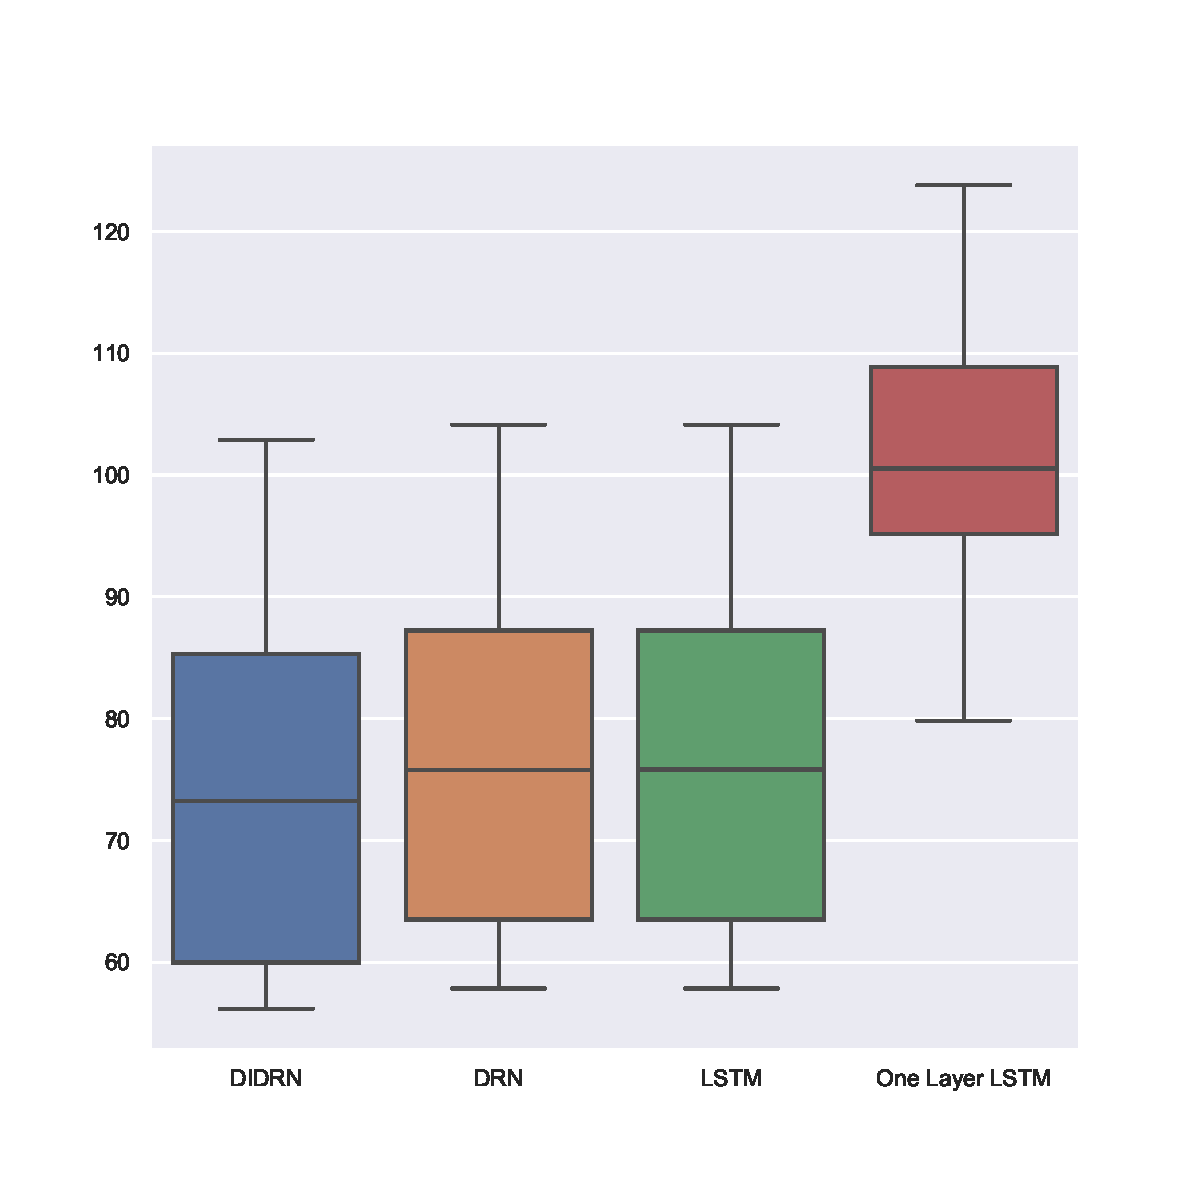
\includegraphics[width = 5cm]{Figure/Box_RMSE.pdf}
}
\subfigure[MAE]{
	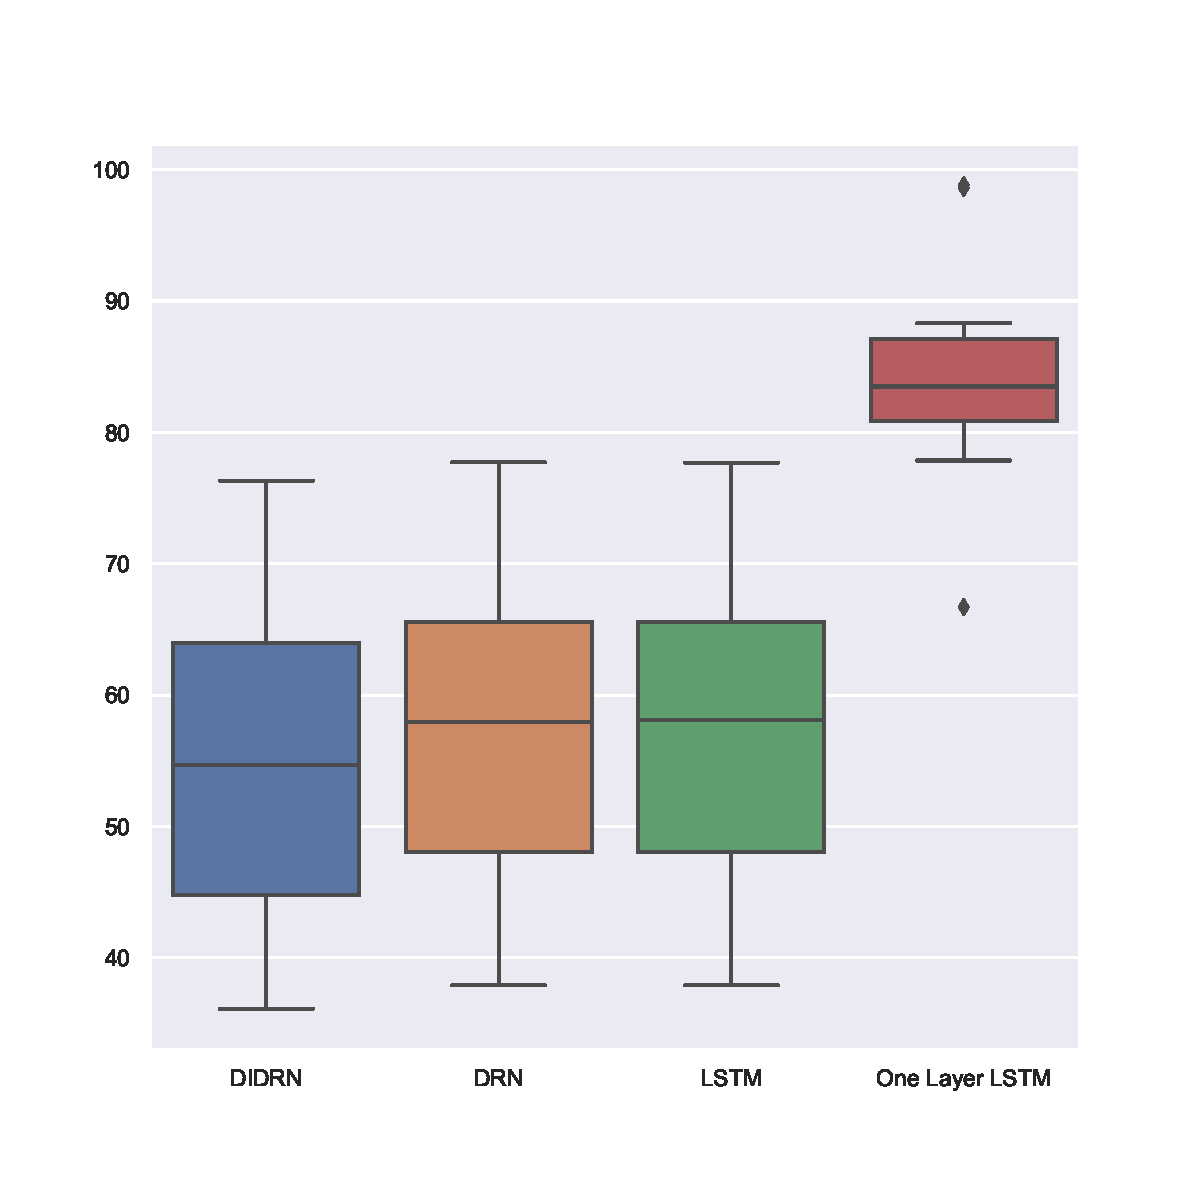
\includegraphics[width = 5cm]{Figure/Box_MAE.pdf}
}
\caption{Forecast Error of Different Models}
\label{fig:box}
\end{figure*}

\par
Table \ref{tab:1} showed that DIDRN obtained performance than the other models. One layer LSTM obtained the worst performance among the models because of its shallow depth. Deep LSTM achieve satisfactory performance. However, on our machine, it actually takes nearly 5 minutes to process data from one detector and train it before it converges. DRN, which was significantly easier to train, obtained a similar but lower error rate than deep LSTM. DRN only takes us about 50 seconds to train. By contrast, although DIDRN was derived from DRN, it achieved a lower error rate than DRN, thereby indicating that our model was efficient enough and training was easy. We could complete the training process within 100 seconds which was slightly longer than that of DRN but was significantly shorter than that of deep LSTM. DRN and Deep LSTM obtained similar performance results because both are comparably accurate when the network is not deep enough \citep{DRN}. This result was similar to those demonstrated in their study. When the network became very deep, their variation would be revealed. But generally, DRN needs less time to be trained.
\par
Table \ref{tab:1} presents that the model accuracy of dataset 4050 is significantly lower than those of other datasets. We plot the data points of dataset 2010 and dataset 4050 as shown in Fig \ref{fig:goodbad}. The shadow represented the range of traffic flow at each time point and the solid line denoted the mean traffic flow value of that time point. The figure showed that the more discrete data in dataset 4050 was not as stable as those of other dataset.  The evaluated models generally obtained poor performance in this type of circumstance.

\begin{figure*}[t]
    \centering
    \subfigure[Dataset 2010]{
    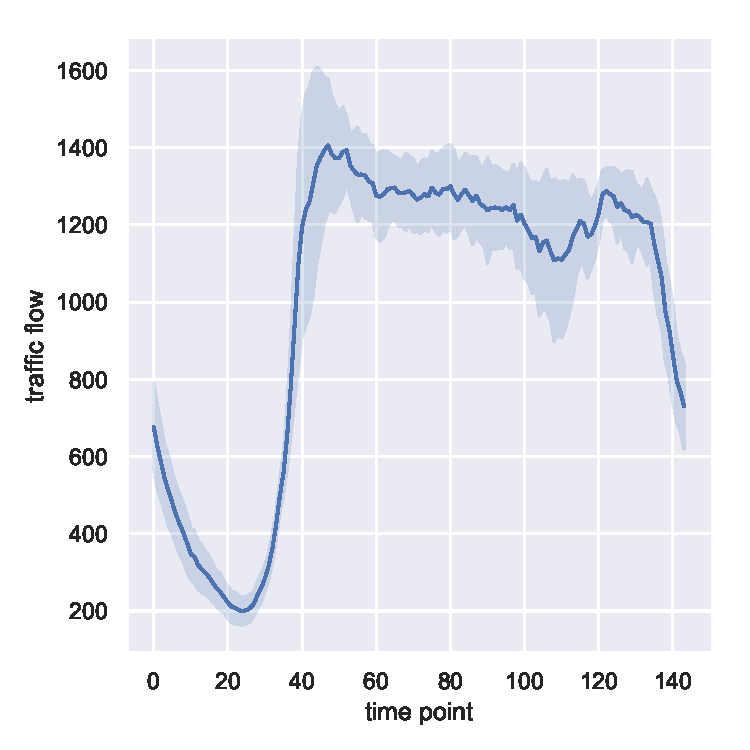
\includegraphics[width=5cm]{Figure/goodOne.pdf}
    }
    \subfigure[Dataset 4050]{
    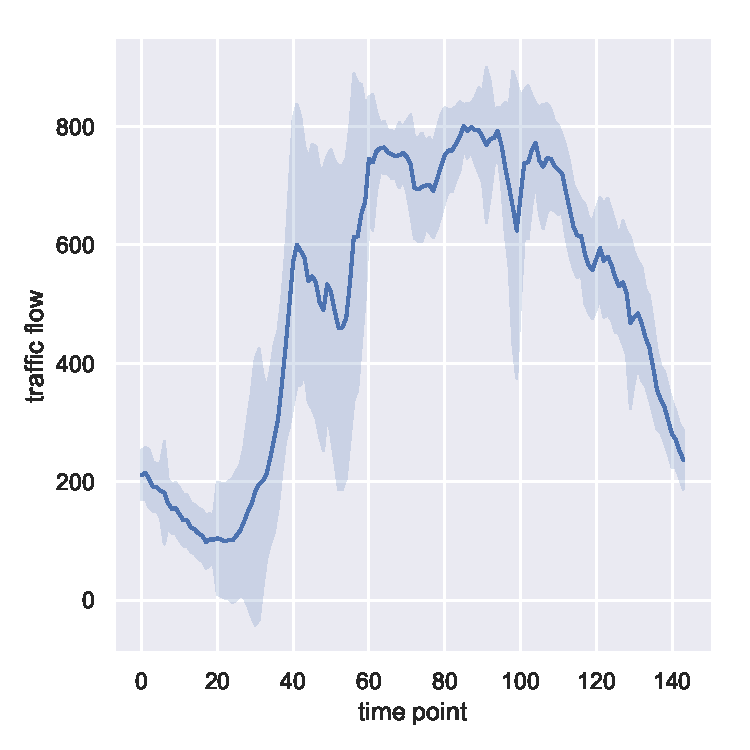
\includegraphics[width=5cm]{Figure/badOne.pdf}
    }
    \label{fig:goodbad}
\end{figure*}


Figure~\ref{fig:measure} shows the comparison of predicted data and measured data in DIDRN and dataset 2010, respectively.
\begin{figure*}[t]
    \centering
    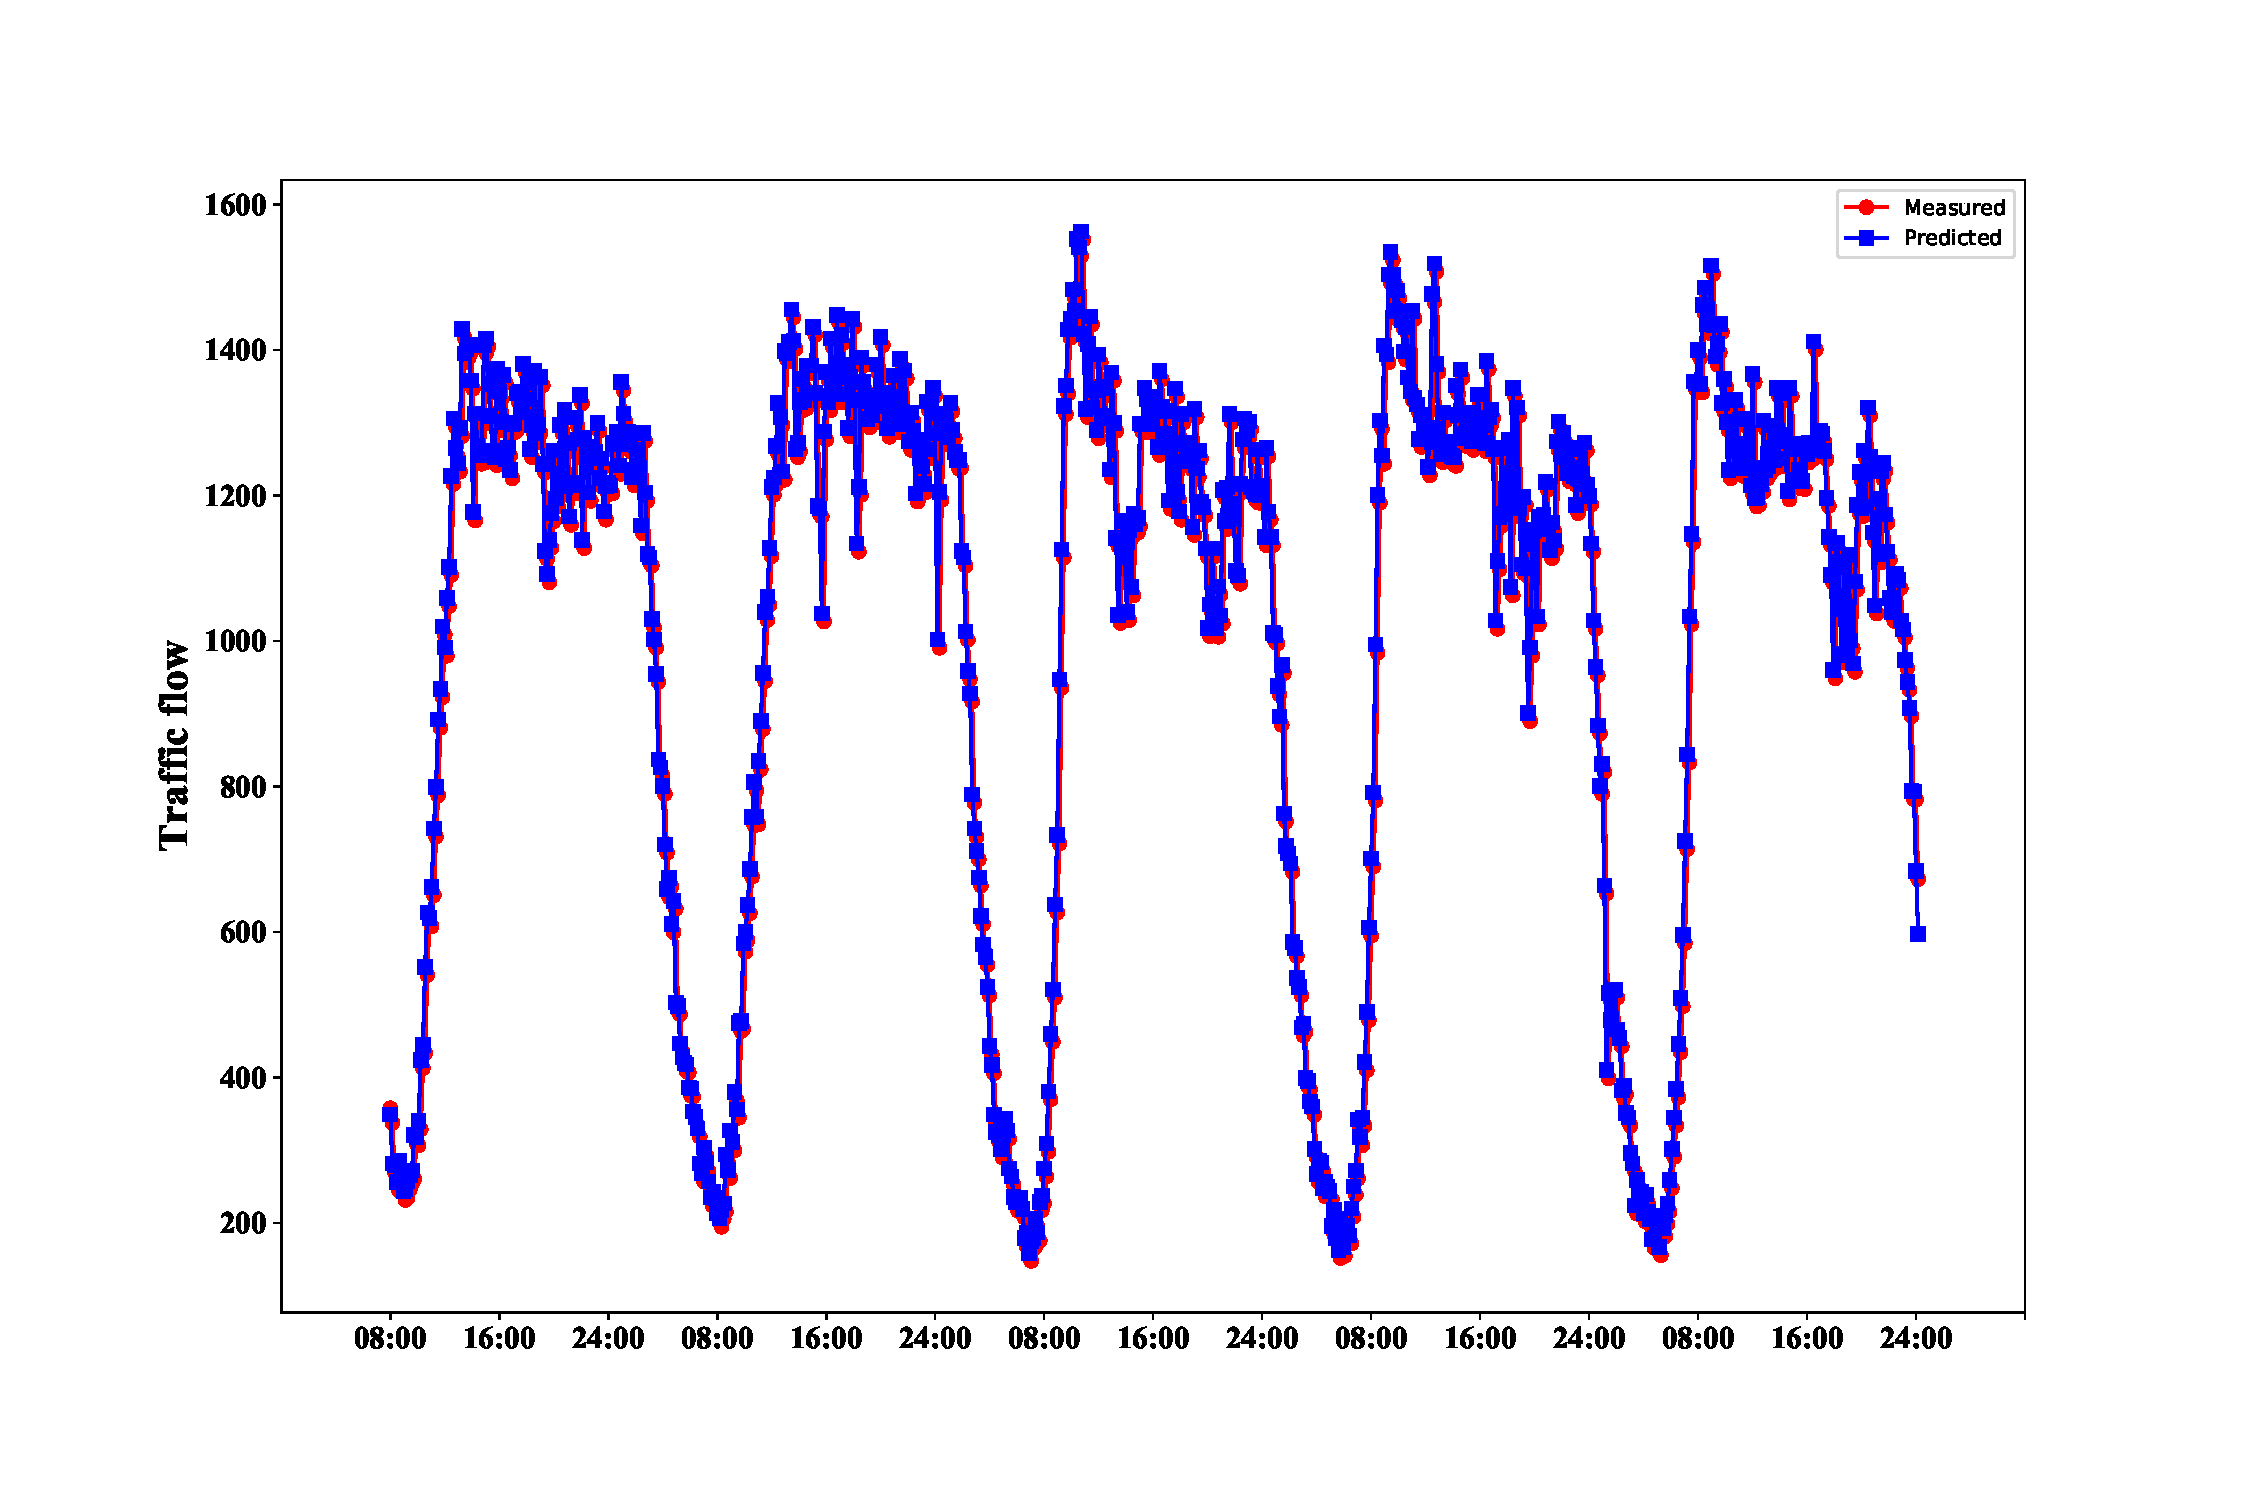
\includegraphics[width=12cm]{Figure/pre.pdf}
    \caption{Measured data and predicted data}
    \label{fig:measure}
\end{figure*}

\subsubsection{Further Analysis on Performance of DIDRN}\label{subsubsec:further}
\par
The experiments were conducted under the following motivations:
\begin{enumerate}[(1)]
    \item Our model showed good performance when the chosen time interval was 10 minutes. However, a model commonly obtains poor performance when the time interval is enlarged. We were motivated to perform an in-depth investigation on the impact of time interval on model performance.
    \item Table~\ref{tab:1} shows that when time interval is 10 minutes, the MAPE is satisfactory. However, we aimed to determine experimentally in this section if our model can obtain even better performance by using another time interval.
    \item The practical scenario was far more complicated than the theoretical one. A problem occured when our model obtained the best performance theoretically at the time interval of 10 minutes. However, in practice, the detector could only provide us the data with a time interval larger than 10 minutes. The third motivation in this section led to the following questions: how did our model perform by using that data? Can we use the data obtained from 1 day or 1 week ago if these are the only data available? What is the accuracy of our model under these conditions.
\end{enumerate}

\par
In the following discussion, our analysis was conducted mainly based on MAPE because of its simplicity and intuitiveness. The data of detector 2010 were chosen to demonstrate the results by using random selection. However, data from either detectors would show similar results.

\par
To evaluate the stability of our proposed model, we changed the time step from 10 minutes to 1 hour with a time interval of 10 minutes, 2 hours, and 24 hours. Moreover, DIDRN was used to conduct the experiments.

\begin{table*}
 \centering
    \caption{Performance of DIDRN on Different Time Intervals}
    \label{tab:3}
    \begin{tabular}{cccc}
    \toprule
    Time Interval (minutes) & RMSE & MAPE & MAE\\
    \midrule
    10 & 75.04 & 6.43\% & 56.43\\
    20 & 119.39 & 11.58\% & 91.77\\
    30 & 128.11 & 11.35\% & 93.01\\
    40 & 198.34 & 19.61\% & 153.16\\
    50 & 197.69 & 17.26\% & 140.90\\
    60 & 202.87 & 18.45\% & 141.34 \\
    120 & 342.96 & 32.67\% & 233.05 \\
    1440 & 135.24 & 10.88\% & 94.92 \\
    \bottomrule
    \end{tabular}
\end{table*}
\begin{figure*}
\centering
\subfigure[MAPE]{
	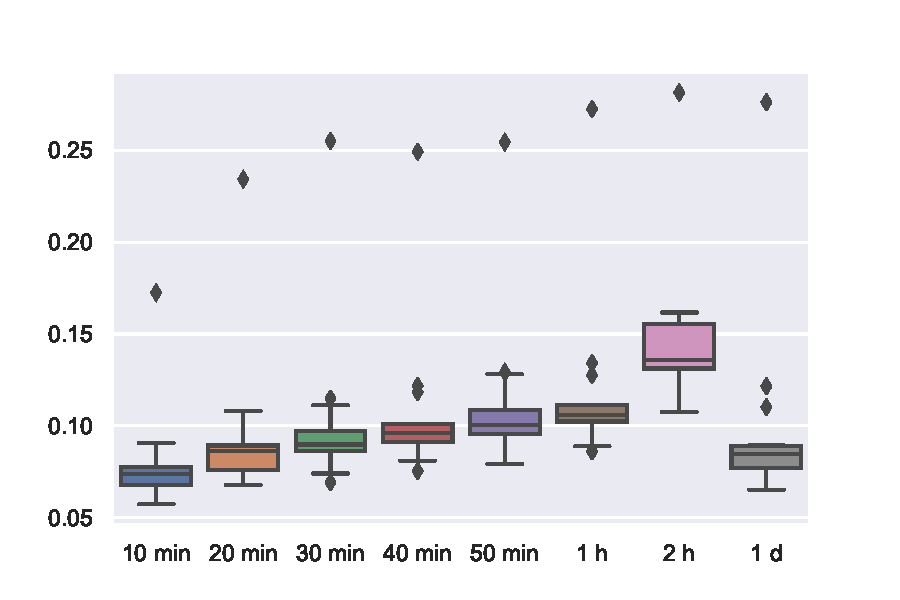
\includegraphics[width = 5cm]{Figure/MAPE-BOX-DARK.pdf}
}
\subfigure[RMSE]{
	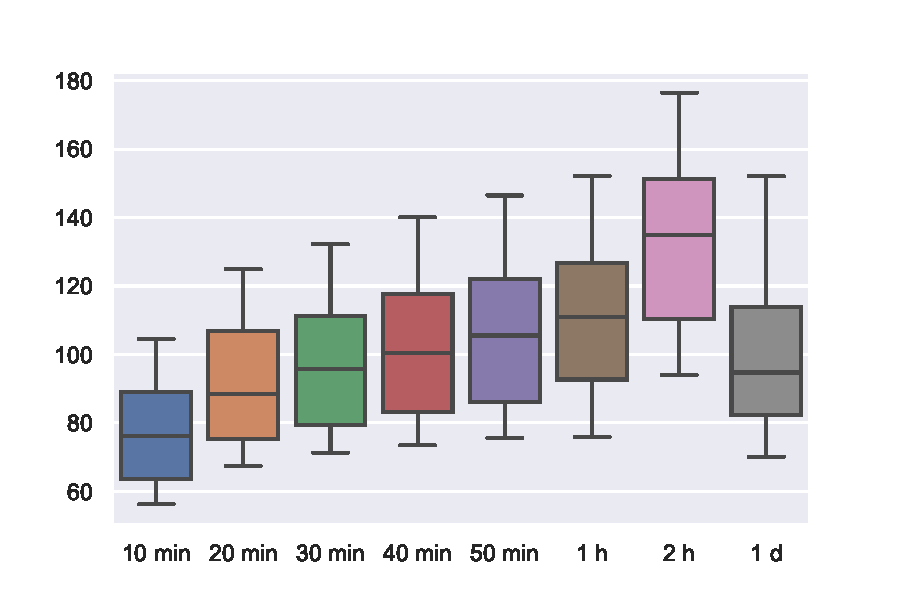
\includegraphics[width = 5cm]{Figure/RMSE-BOX-DARK.pdf}
}
\subfigure[MAE]{
	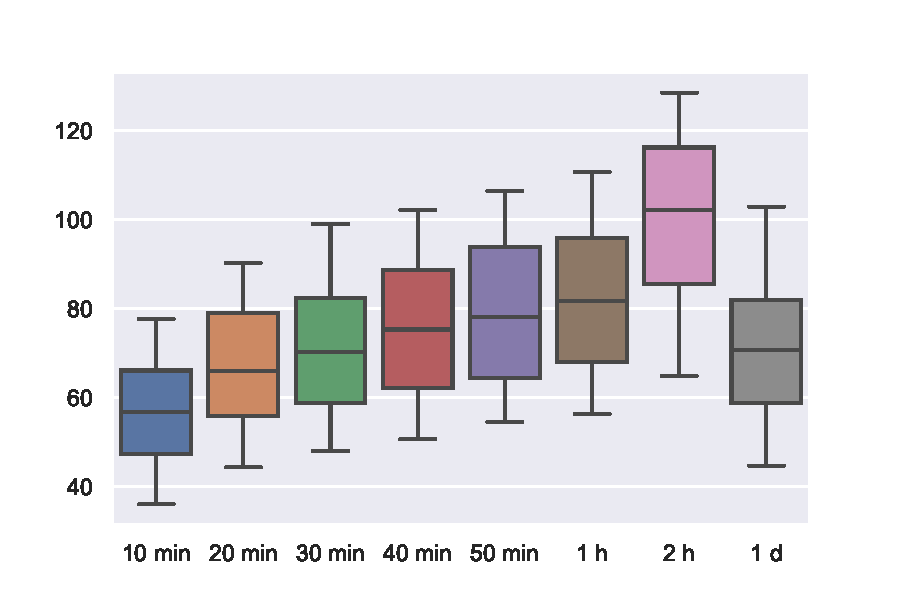
\includegraphics[width = 5cm]{Figure/MAE-BOX-DARK.pdf}
}
\end{figure*}
\par
Table~\ref{tab:3} shows that accuracy decrease monotonously when the time interval increases from 10 minutes to 1 hour and 2 hours, the accuracy decreases monotonously. This result is congruent with our intuition. When the time interval became larger, we needed more information to predict the traffic flow and the traffic flow of the previous time point is less related to the traffic flow of the predicted time point. Therefore, accuracy was reduced. However, when we use the traffic flow of the previous day to predict that of the next day, accuracy significantly increased to 10.88\% in terms of MAPE. On one hand, traffic flow data are stable with a periodic nature\citep{tan2013tensor,tan2016comparison,wu2017robust}. Thus, the traffic flow of the same time in the previous day was relatively similar to that of the predicted day, especially when two consecutive workdays were considered. On the other hand, traffic flows after 1 or 2 hours could be significantly different with those of the current time point. For example, the traffic flow at 7:00 a.m. was significantly different compared with that at the peak hours of 8:00 a.m. and 9:00 a.m. People go to work during peak hours, thereby leading to a sudden increase in traffic flow. As the only input was data from 7:00 a.m. when the model attempted to predict the traffic flow at 8:00 a.m. or 9:00 a.m., the model did not have enough information to predict this sudden increase. Hence, the predicted values obtained a larger deviation from the detected values.



\par
Table~\ref{tab:4} lists the MAPE values of different detectors in terms of predicting 1 day in advance. Hence, we used the data of the previous days to predict the traffic flow of the next day. The results revealed that the model obtained a stable performance from data of different detectors. The model achieved poor performance from data of detector 4050 because the corresponding data of this detector were not fluctuant. That is, the traffic flow obtained by the detector in this location was unstable over time. Our model could not be expected to perform well when the data were not good and stable enough. This observation was supported by the results shown in Table~\ref{tab:1}.

\begin{table*}
 \centering
    \caption{One day forward prediction accuracy of different detectors}
    \label{tab:4}
    \begin{tabular}{ccccccccccccccc}
    \toprule
    Detector & 2010 & 2011 & 2013 & 2023 & 2030 & 2033 & 2052 \\
MAPE & 10.88\%
&12.64\% &
15.01\% &
10.66\% &
10.74\% &
9.43\% &
12.31\%\\

\midrule
Detector & 3034 & 3035 & 4004 & 4005 & 4050 & 4051 & 5062 \\
MAPE & 10.71\% &
10.50\% &
11.35\% &
9.83\% &
52.40\% &
33.60\% &
12.27\% \\
    \bottomrule
    \end{tabular}
\end{table*}

\par
To further analyze the impact of time interval, we gradually increased the time interval from 1 to 7 days. 
\par 
Table~\ref{tab:11} shows the results. When the time interval ranged from 2 to 6 days, the error rate ranged from 13.96\% to 10.45\%. Because the predicted traffic flow had reduced relation with the input traffic flow when the time interval increased. The model had less information to update its weights and perform well in both training set and test set.
\par
A large increase occurred between 6 and 7 days. Owing to symmetry, the error rate of 6 days should be similar to that of 1 day, which was also consistent with our results. As traffic flow data are a type of periodic data and the period was exactly 7 days, it is not surprising that the flow 1 week later is similar to the current flow. Owing to this property, our model obtained better performance and higher accuracy than the others.

\begin{table*}
 \centering
    \caption{Performance of DIDRN for weekday and weekend}
    \label{tab:11}
    \begin{tabular}{cccc}
    \toprule
    Days & RMSE & MAPE & MAE\\
    \midrule
    1 &135.24 &10.88\% & 94.92 \\
    2 &158.27 &13.96\% &113.70 \\
    3 &154.55 &13.81\% &109.36 \\
    4 &145.62 &13.22\% &104.54 \\
    5 &142.73 &10.85\% &99.14 \\
    6 &143.36 &10.45\% &98.12 \\
    7 &100.56 &7.28\% &69.48 \\
    \bottomrule
    \end{tabular}
\end{table*}

\par
We increased the time interval from 10 minutes to 2 hours and compared the performance with the presented results. In this study, the kind of time interval, which the performance is better when time interval is less than it and the performance is worse when time interval is greater than it, is referred as boundary time (BT). Figure \ref{fig:12} shows the results of time intervals at less than 2 hours, 1 day and 7 days.
This figure illustrated that MAPE increased when the time interval increased. The best performance was obtained by our model when time interval is equal to 10 minutes.  The performance of 1 day was better than that of 30 minutes but was worse than 20 minutes, whereas the performance of 1 week was better than that of 20 minutes but was worse than that of 10 minutes. This experiment was also conducted on data from the other detectors. Table~\ref{tab:13} lists the boundary time for all detectors.
\begin{table*}
    \centering
    \caption{Boundary Time of All Detectors (BT(1 day) represents the BT with respect to MAPE of 1 day)}
    \begin{tabular}{ccccccccccccccc}
    \toprule
     Detector    & 2010 & 2011 & 2013 & 2023 & 2030 & 2033 & 2052 \\
      BT(1 day) /min  & 30 & 30 & 40 & 20 & 20 & 20 & 30 \\
      BT(1 week) /min & 10 & 10 & 10 & 20 & 10 & 10 & 10\\
      \midrule
     Detector & 3034 & 3035 & 4004 & 4005 & 4050 & 4051 & 5062 \\
     BT(1 day) /min & 30 & 20 & 40 & 30 & 120 & 70 & 30\\
     BT(1 week) /min & 10 & 10 & 10 & 20 & 60 & 60 & 10\\
      \bottomrule
    \end{tabular}
    \label{tab:13}
\end{table*}

\par
On the basis of these results, the following conclusions could be drawn:
\begin{enumerate}
    \item If data of the previous time point were available, then using those data to predict traffic flow of next time point was the best option. That is, the time interval should be set to 10 minutes.
    \item If data of the previous week were available or the task was to conduct long-term prediction, then using these data was better.
    \item When the time interval was greater than 30 minutes, the performance was generally better than 1 day or 1 week time intervals. In practical applications, BT could be obtained by using historical data, which could be used as a reference for choosing the time interval in predicting the traffic flow. 
\end{enumerate}
\begin{figure*}
    \centering
    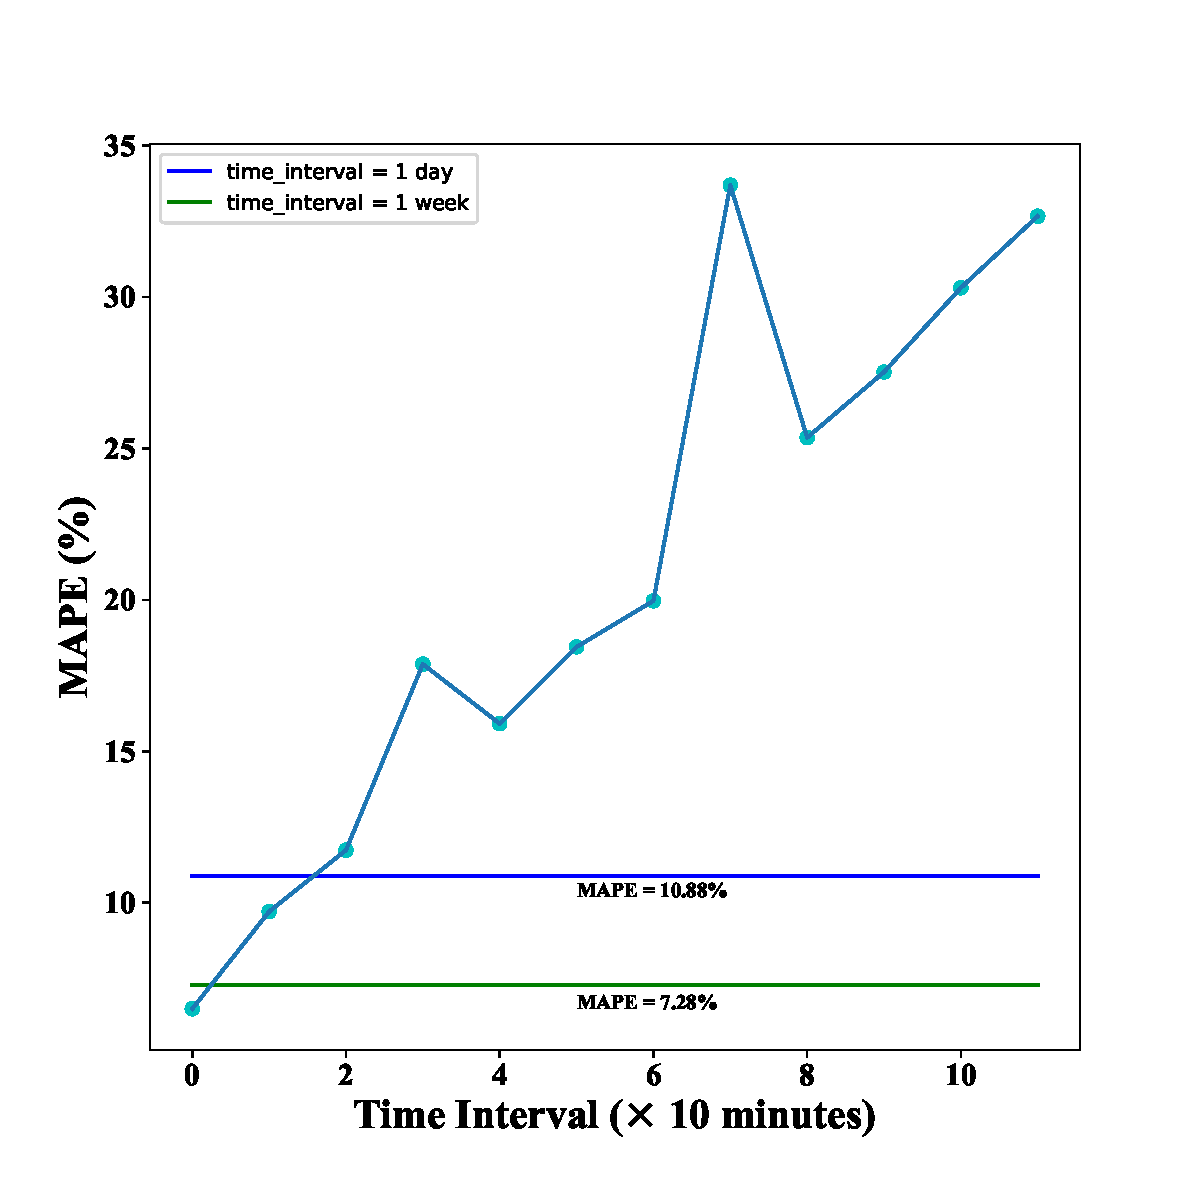
\includegraphics[width = 8cm]{Figure/Bound.pdf}
    \caption{MAPE for Different Time Intervals}
    \label{fig:12}
\end{figure*}

\section{Conclusion and Future work} \label{sec:confw}

In this study, we demonstrated the basic concepts of deep residual network. The results showed that DRN was much simpler to train and obtained better performance than other approaches. We then explain the motivations and improvements of DRN in our research. We showed the architecture of our network and how it works. Finally, we proposed our dynamic model DIDRN and demonstrated why it makes sense.
\par
We presented the steps of processing data. We explained how raw data was processed into data that can be used in supervised learning and how we obtained the final predictions. Then, we performed several experiments and compared the performance of the different models. The results showed that DIDRN exhibited better performance than other commonly used models. From the view of MAPE, DIDRN obtained a maximum of 1.41\% performance improvement compared to LSTM and DRN.  From the view of RMSE and MAE, DIDRN achieved a maximum reduction of 9.

\par
On the basis of these results, we analyzed our model by changing the time interval which is an input value and implemented the multi-step forward prediction which verifies the stability of our model. On the basis of performance at different time intervals, we demonstrated a recommended BT which could be a good choice in predicting traffic flow via the proposed model.


\par
Despite the good performance, our model still exhibited some shortcomings. We only considered temporal pattern in this study. In future research, the spatial pattern would be considered and we will investigate spatial-temporal dependence in our model. 
\par
In addition, our model could perform traffic flow prediction well when the time interval or the period of our data was small. However, our model obtained poor performance when the time interval was slightly large. Future studies could be carried out to extend the model into a generalized version and obtain good performance when the time interval is both small and large, thereby indicating efficiency in both short-term and long-term traffic flow predictions.


\bibliographystyle{plainnat}
\bibliography{Reference.bib}


% \appendix
\begin{appendices}
\section{Algorithms}\label{algorithms}
\begin{algorithm}[htbp]
\SetAlgoLined
\SetKwInOut{Input}{Input}\SetKwInOut{Output}{Output}
\SetKwData{Data}{Data}
\caption{TimeSeriesToSupervised($R,lag)$}
\label{alg:a2}
\BlankLine
\tcp{R: data returned by function \texttt{Difference}}
\tcp{$lag$: lag is the number of time points used to predict data of next time point, in our research, lag = 1}
shiftedData = shift $R$\;
$R$.append(shiftedData)\;
return $R$;
\end{algorithm}

\begin{algorithm}[htbp]
\SetAlgoLined
\SetKwInOut{Input}{Input}\SetKwInOut{Output}{Output}
\SetKwData{Data}{Data}
\caption{Difference$(D,interval)$}
\label{alg:a1}
\BlankLine
\tcp{$D$: raw data}
\tcp{$interval$: time interval}
Initialize $R$ as $\emptyset$\;
\For{i from interval to D.length}{
    $D$.append($D[i] - D[i-interval]$)\;
}
return $R$;
\end{algorithm}

\begin{algorithm}[htbp]
\SetAlgoLined
\SetKwInOut{Input}{Input}\SetKwInOut{Output}{Output}
\SetKwData{Data}{Data}
\caption{inverseDifference($historyData,\Hat{y},interval$)}
\label{alg:a3}
\BlankLine
\tcp{$historyData$: data used in \texttt{Difference}}

\tcp{$\Hat{y}$: the predicted difference of normalized traffic flow volume between two data points}
\tcp{$interval$: time interval}
Initialize $D$ as $\emptyset$\;
$D = \Hat{y} + history[-interval]$\;
\tcp{$history[-i]$ represents the last $i^{th}$ data point}
return $D$;
\end{algorithm}

\begin{algorithm}[htbp]
\SetAlgoLined
\SetKwInOut{Input}{Input}\SetKwInOut{Output}{Output}
\SetKwData{Data}{Data}
\caption{scaleData($trainData,testData$)}
\label{alg:a4}
\BlankLine
\tcp{$trainData$: training data}
\tcp{$testData$: test data}
$Max_1 = trainData.max$ $\quad Min_1 = trainData.min$\;
$Max_2 = testData.max$ $\quad Min_2 = testData.min$\;
Initialize $TD_1,TD_2$ as $\emptyset$\;
\For{each data point $DP_1$ in $trainData$}{
    $newDP_1 = \frac{DP_1-Min_1}{Max_1-Min_1}$
    $TD_1$.append($newDP_1$)\;
}
\For{each data point $DP_2$ in $testData$}{
    $newDP_2 = \frac{DP_2-Min_2}{Max_2-Min_2}$
    $TD_2$.append($newDP_2$)\;
}
return $TD_1$ and $TD_2$;
\end{algorithm}

\begin{algorithm}[htbp]
\SetAlgoLined
\SetKwInOut{Input}{Input}\SetKwInOut{Output}{Output}
\SetKwData{Data}{Data}
\caption{MainAlgorithm($D$)}
\label{alg:a5}
\BlankLine
\tcp{$D$: raw data}
Set all parameters;
$DV  = \texttt{Difference(D)}$\;
$SV = \texttt{timeSeriesToSupervised}(DV)$\;
Split SV into training set $TS_1$ and test set $TS_2$\;
Scale $TS_1,TS_2$\;
Use scaled $TS_1$ to train the model\;

Initialize the set of predict values $PV$ as $\emptyset$\;
\For{each time point $tp$ in $TS_2$}{
    Use trained model to predict value at $tp$\;
    Add predicted value to $PV$\;
    Add $TS_2(tp)$ to $TS_1$\;
    Incrementally train model\;
}
Calculate error rate\;
\end{algorithm}
\end{appendices}
\end{document}

$ .tex
$ .bib
$ .tex
$ .tex
